\chapter{Mininet-Wifi}

Por lo que he leído Mininet-Wifi no incorpora el estándar que usábamos para el estudio de las redes de área personal con tasa baja de transmisión de datos, 802.15.4 .
\section{Enlaces útiles}
\begin{itemize}
    \item Articulos sobre Mininet y Mininet-Wifi: \url{http://www.brianlinkletter.com/tag/mininet/}
    
\end{itemize}


\section{¿Qué es?}


Mininet-Wifi es un fork del proyecto Mininet con el que podías emular redes SDN, y se han extendido sus funcionalidades al ámbito de las redes wireless. Por lo que con el se pueden combinar ambas funcionalidades, las anteriores comunes a Mininet y las nuevas que incorpora Mininet-Wifi.

\section{¿Qué es el término RSSI?}

El indicador de fuerza de la señal recibida (RSSI por las siglas del inglés Received Signal Strength Indicator), es una escala de referencia \textbf{en relación a 1 mW} para medir el nivel de potencia de las señales recibidas por un dispositivo en las redes inalámbricas (típicamente WIFI o telefonía móvil).



% Please add the following required packages to your document preamble:
% \usepackage{booktabs}

\begin{table}[!htb]
\centering
\begin{tabular}{@{}ll@{}}
\toprule
RSSI & Descripción                                                                                                                                                        \\ \midrule
0    & Señal ideal                                                                                                                                                        \\
-40  & Señal idónea con tasas de transferencia estables.                                                                                                                  \\
-60  & \begin{tabular}[c]{@{}l@{}}Enlace bueno, ajustando la \\ transmisión (Tx) se puede lograr una conexión estable al 80\%\end{tabular}                                \\
-70  & \begin{tabular}[c]{@{}l@{}}Enlace medio-bajo, es una señal medianamente buena\\ aunque se pueden sufrir problemas con lluvia y viento.\end{tabular}                \\
-80  & \begin{tabular}[c]{@{}l@{}}Es la señal mínima aceptable para establecer la conexión.\\ Pueden ocurrir caídas que se traducen en corte de comunicación\end{tabular} \\ \bottomrule
\end{tabular}
\centering 
\end{table}

\newpage

\section{Instalación}

Instalar Mininet-Wifi me ha resultado muy sencillo. Se lleva a cabo vía un shellscript que te dan ya hecho al clonar el repositorio de Mininet-Wifi. Los pasos que he seguido en la instalación de Mininet-Wifi son:
\begin{itemize}
    \item Instalar una máquina virtual con Ubuntu 16.04
    \item Añadir git, sudo apt-get install git 
    \item Clonar el repositorio, git clone https://github.com/intrig-unicamp/mininet-wifi
    \item cd mininet-wifi
    \item Completar la instalación: sudo \textbf{util/install.sh -Wlnfv}
    \begin{itemize}
        \item -W: wireless dependencies
        \item -n: mininet-wifi dependencies
        \item -f: OpenFlow
        \item -v: OpenvSwitch
        \item -l: wmediumd
    \end{itemize}
    \item De forma adicional hemos instalado Wireshark para poder analizar los test realizados
\end{itemize}

\section{Test 1}
La red más sencilla es por defecto la red de un punto de acceso y dos estaciones wireless. El punto de acceso está conectado directamente al controlador, y las estaciones wireless serán los host. La idea de este test es comprobar que hay fluctuación de tráfico de control OpenFlow en el punto de acceso y además hay tráfico de usuario en la interfaz de wlan.

\begin{itemize}
    \item Lanzamos Wireshark para analizar tráfico: \textbf{wireshark \&}
    \item Lanzamos Mininet-Wifi con el siguiente comando, además por defecto cargará la topología por defecto(Valga la redundancia): \textbf{sudo mn -wifi}
    \item Lo siguiente, es activar la interfaz hwsim0. Pero, ¿Qué es la interfaz hwsim0? La interfaz hwsim0 es una interfaz software creada por Mininet-Wifi que copia todo el trafico wireless  dirigido a todas las interfaces wireless virtuales de la topología a emular. Según la documentación seguida es la forma más sencilla de monitorizar los mensajes wireless en Mininet-Wifi. Desde la Mininet-Wifi CLI: \textbf{sh ifconfig hwsim0 up} 
    \begin{itemize}
        \item El comando \textbf{sh} en la CLI de Mininet tiene la funcionalidad de ejecutar un comando fuera de la Interfaz de Mininet-Wifi.
    \end{itemize}
    
    \item Una vez levantada la interfaz podemos poner Wireshark a escuchar en la interfaz.
    
    \item Hacemos Ping desde la estación sta1, a la estación sta2: \textbf{sta1 ping sta2}
    
    \item Comprobamos que hay tráfico escuchando en la interfaz:
    
    
\end{itemize}
\newpage
\begin{figure}[!htb]
  \centering
    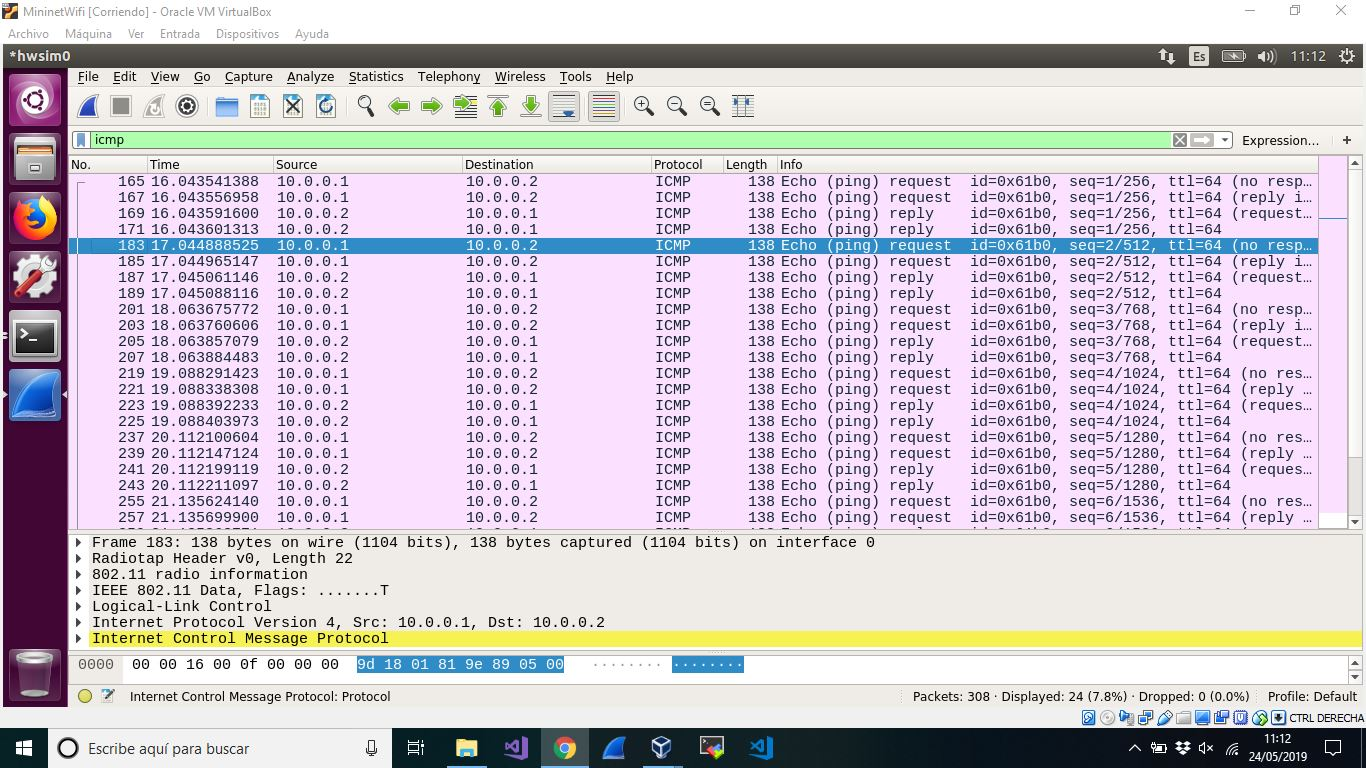
\includegraphics[width=\linewidth]{./img/5.JPG}
    \caption{Comprobación que hay trafico a través de la interfaz.}
  \label{fig:yo}
\end{figure}

Como podeos ver el punto de acceso tiene una interfaz asociada llamada ap1-wlan1. Por defecto, las estaciones wireless asociadas con el punto de acceso se conectan en modo "\textbf{infrastructure} " esto significa que el tráfico wireless entre dos estaciones asociadas al punto de acceso debe pasar siempre a través de este. Sabiendo que los puntos de acceso funcionan de forma similar a los switch en Mininet, esperaríamos observar tráfico de control entre el punto de acceso y el controlador, cuando el punto de acceso,  observe tráfico para el cual no se establecido una regla (No pertenece a un flujo para el cual haya asignada una acción en la tabla de flujos). 

\begin{figure}[!htb]
  \centering
    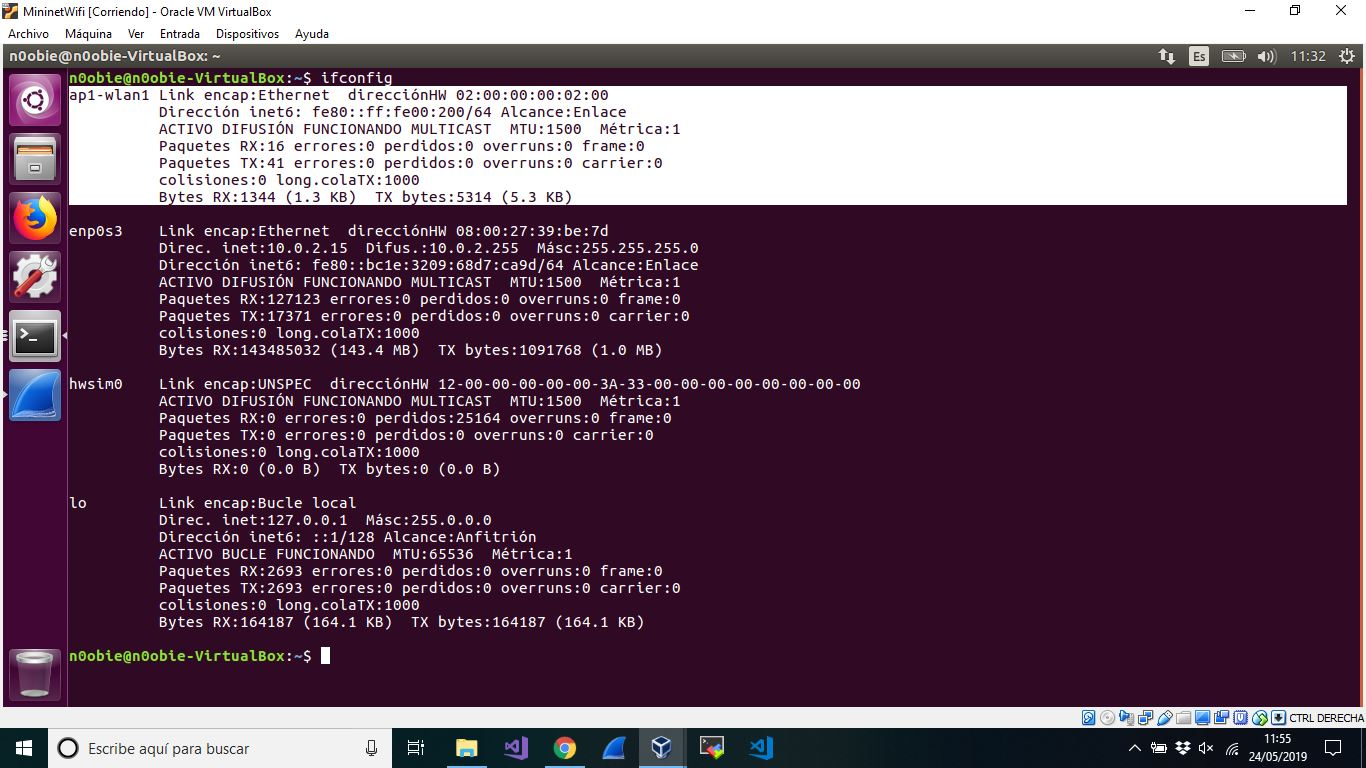
\includegraphics[width=0.9\linewidth]{./img/6.JPG}
    \caption{Interfaz ap1-wlan1 del Punto de acceso.}
  \label{fig:yo}
\end{figure}
\newpage
Si deseamos ver \textbf{paquetes OpenFlow}, debemos poner a escuchar Wireshark  en la interfaz de \textbf{loopback}. Podemos además utilizar el filtro: \textbf{OpenFlow\_1.0} para visualizarlo de una forma más clara. Dicho esto, ponemos a capturar Wireshark y repetimos el ping entre sta1 y sta2.
\begin{figure}[!htb]
  \centering
    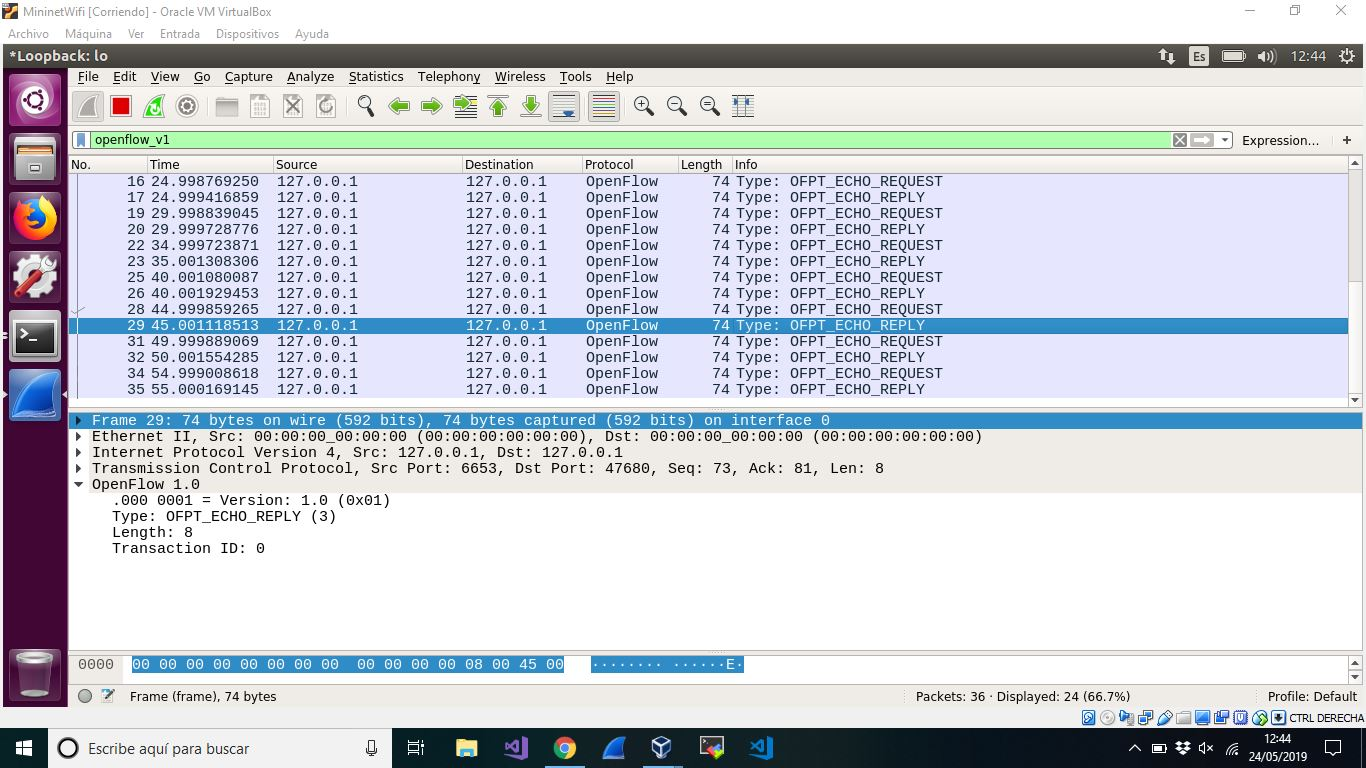
\includegraphics[width=\linewidth]{./img/7.JPG}
    \caption{Tráfico OpenFlow.}
  \label{fig:yo}
\end{figure}
\newline
Nota: 
\begin{itemize}
    \item Consultar comando dpctl: \url{http://ranosgrant.cocolog-nifty.com/openflow/dpctl.8.html}
    \item xID: Identificador de transacción, es aleatorio, identificador controlador - switch, va cambiando a lo largo del tiempo.  
    \item El estándar es OpenFlow 1.3, pero Mininet-Wifi funciona con OpenFlow 1.1
\end{itemize}

Como esperábamos el paquete ICMP debería ser redirigido al controlador para decidir que hacer con el paquete, al no tener un Flow con una regla establecida. De esta manera el controlador cuando  le llegue el paquete instanciará una serie de reglas en los switch para que el paquete ICMP sea encaminado de un host a otro. En cambio, encontramos que las dos estaciones son capaces de intercambiar paquetes inmediatamente sin redirigir el primer paquete al controlador. Solo una trama ARP , que es de tipo broadcast, es llevada hacia el controlador y es ignorada.\newline
\newline
Para comprobar si hubira algún flujo con una ccción instanciada en alguna de las estaciones bases hacemos:
\textbf{dpctl dump-flows}
\newline
\newline
Al hacer esto en esta altura del tutorial, vemos que no hay ninguna regla instanciada en la estación. ¿Pero, tiene esto sentido?¿Cómo se han comunicado las dos puntos de acceso?\newline
\newline
Según la guía, podemos apreciar que los switches con OpenFlow activado, van a rechazar las "Hairpin connections". Las cuales son flows que hacen que el tráfico, sea enviado por el mismo puerto que ha sido recibido.

\begin{itemize}
    \item \textbf{Hairpin connection}: Comunicación entre dos dispositivos host en el mismo dominio NAT utilizando sus puertos finales(Ya traducidos)
\end{itemize}
\newpage
\begin{figure}[!htb]
  \centering
    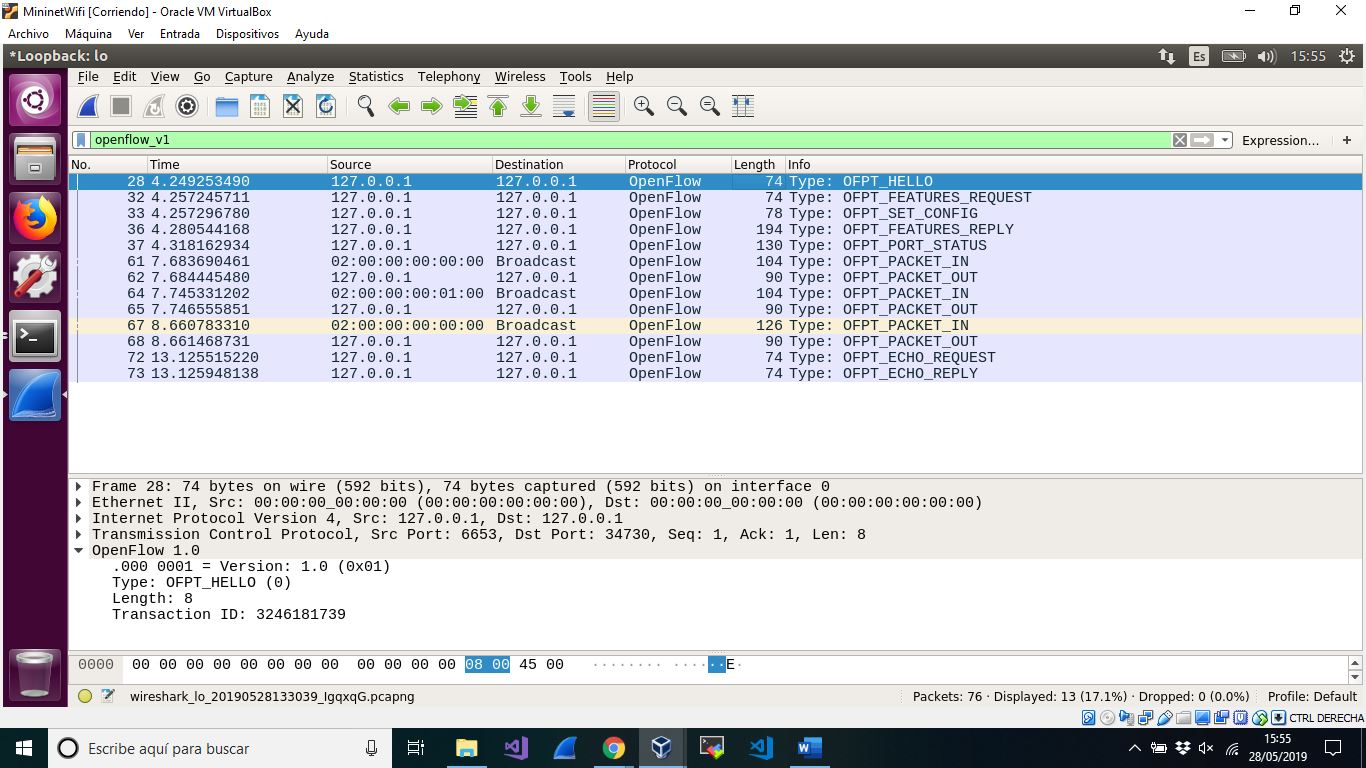
\includegraphics[width=\linewidth]{./img/8.JPG}
    \caption{No hay tráfico OpenFlow hacia el controlador.}
  \label{fig:yo}
\end{figure}
Un punto de acceso wireless, por diseño, recibe y manda paquetes en la misma interfaz. Las estaciones wifi conectadas al mismo punto de acceso requerirán a "Hairpin connection" para comunicarse entre ellas. El autor de la guía supone que Linux, maneja a la interfaz WLAN en cada punto de acceso como un enlace radio sta1-ap1-sta2 como si fuera un HUB, donde ap1-wlan0 proporciona la funcionalidad de "HUB"
para los datos que pasan entre sta1 y sta2.
ap1-wlan0 cambia los paquetes en el dominio inalámbrico y lo hará
no introduzca un paquete en la parte del "conmutador Ethernet" del punto de acceso ap1 a menos que deba cambiarse a
otra interfaz en ap1 que no sea ap1-wlan0.\newline
\newline
\begin{itemize}
    \item Podemos detener el ping con CTRL+C
    \item Podemos detener Mininet-Wifi vía comando \textbf{exit}
    \item Podemos limpiar los archivos residuales de Mininet-Wifi con:  \textbf{sudo mn -c}
\end{itemize}

\section{Test 2}
En este test vamos a crear una topología lineal con tres puntos de acceso, y tres estaciones wifi. Donde cada una está conectada a cada punto de acceso.\newline
\newline
Podemos crear la topología: \textbf{sudo mn --wifi --topo linear,3}
\newpage
\begin{figure}[!htb]
  \centering
    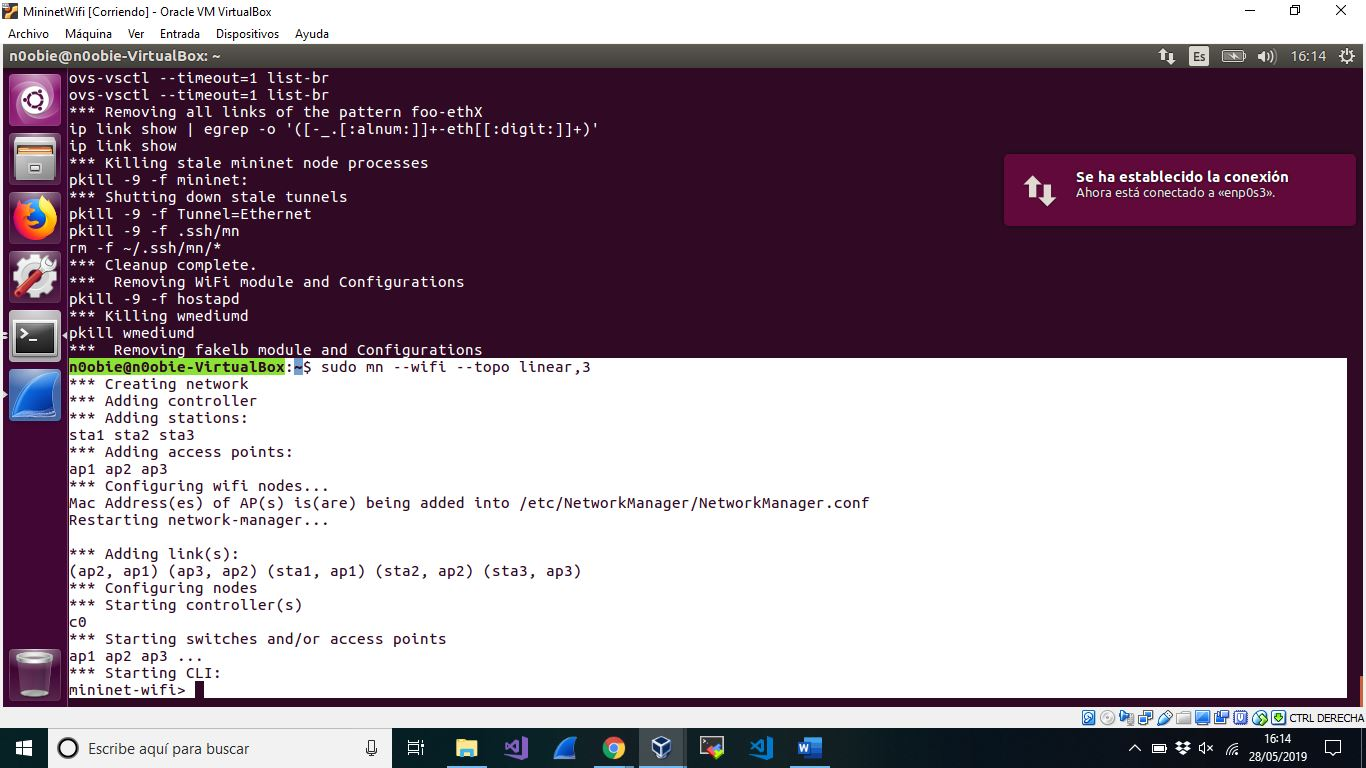
\includegraphics[width=\linewidth]{./img/9.JPG}
    \caption{Montar topología lineal en Mininet-Wifi.}
  \label{fig:yo}
\end{figure}
Además,  podemos  verificar la configuración de la topología haciendo uso de los comandos \textbf{net} y \textbf{dump}. Con el comando \textbf{net} podemos ver la conexión entre los nodos. Con el comando \textbf{dump} podemos ver la conexión entre los nodos y además información extra como el PID.

